\documentclass[xcolor=svgnames]{beamer}\usepackage[]{graphicx}\usepackage[]{color}
%% maxwidth is the original width if it is less than linewidth
%% otherwise use linewidth (to make sure the graphics do not exceed the margin)
\makeatletter
\def\maxwidth{ %
  \ifdim\Gin@nat@width>\linewidth
    \linewidth
  \else
    \Gin@nat@width
  \fi
}
\makeatother

\definecolor{fgcolor}{rgb}{0.345, 0.345, 0.345}
\newcommand{\hlnum}[1]{\textcolor[rgb]{0.686,0.059,0.569}{#1}}%
\newcommand{\hlstr}[1]{\textcolor[rgb]{0.192,0.494,0.8}{#1}}%
\newcommand{\hlcom}[1]{\textcolor[rgb]{0.678,0.584,0.686}{\textit{#1}}}%
\newcommand{\hlopt}[1]{\textcolor[rgb]{0,0,0}{#1}}%
\newcommand{\hlstd}[1]{\textcolor[rgb]{0.345,0.345,0.345}{#1}}%
\newcommand{\hlkwa}[1]{\textcolor[rgb]{0.161,0.373,0.58}{\textbf{#1}}}%
\newcommand{\hlkwb}[1]{\textcolor[rgb]{0.69,0.353,0.396}{#1}}%
\newcommand{\hlkwc}[1]{\textcolor[rgb]{0.333,0.667,0.333}{#1}}%
\newcommand{\hlkwd}[1]{\textcolor[rgb]{0.737,0.353,0.396}{\textbf{#1}}}%

\usepackage{framed}
\makeatletter
\newenvironment{kframe}{%
 \def\at@end@of@kframe{}%
 \ifinner\ifhmode%
  \def\at@end@of@kframe{\end{minipage}}%
  \begin{minipage}{\columnwidth}%
 \fi\fi%
 \def\FrameCommand##1{\hskip\@totalleftmargin \hskip-\fboxsep
 \colorbox{shadecolor}{##1}\hskip-\fboxsep
     % There is no \\@totalrightmargin, so:
     \hskip-\linewidth \hskip-\@totalleftmargin \hskip\columnwidth}%
 \MakeFramed {\advance\hsize-\width
   \@totalleftmargin\z@ \linewidth\hsize
   \@setminipage}}%
 {\par\unskip\endMakeFramed%
 \at@end@of@kframe}
\makeatother

\definecolor{shadecolor}{rgb}{.97, .97, .97}
\definecolor{messagecolor}{rgb}{0, 0, 0}
\definecolor{warningcolor}{rgb}{1, 0, 1}
\definecolor{errorcolor}{rgb}{1, 0, 0}
\newenvironment{knitrout}{}{} % an empty environment to be redefined in TeX

\usepackage{alltt}
\usetheme{Boadilla}
\usecolortheme[named=SeaGreen]{structure}
\usepackage{graphicx}
\usepackage{breqn}
\usepackage{xcolor}
\usepackage{booktabs}
\usepackage{verbatim}
\usepackage{tikz}
\usetikzlibrary{shadows,arrows,positioning}
\definecolor{links}{HTML}{2A1B81}
\hypersetup{colorlinks,linkcolor=links,urlcolor=links}
\usepackage{pgfpages}

\tikzstyle{block} = [rectangle, draw, text width=9em, text centered, rounded corners, minimum height=3em, minimum width=7em, top color = white, bottom color=brown!30,  drop shadow]

\newcommand{\ShowSexpr}[1]{\texttt{{\char`\\}Sexpr\{#1\}}}
\IfFileExists{upquote.sty}{\usepackage{upquote}}{}
\begin{document}

\title[Overview of SWMP data]{SWMP data retrieval and preparation}

\author[M. Beck]{Marcus W. Beck}

\date{}

\institute[USEPA NHEERL]{USEPA NHEERL Gulf Ecology Division, Gulf Breeze, FL\\
Email: \href{mailto:beck.marcus@epa.gov}{beck.marcus@epa.gov}, Phone: 850 934 2480}


%%%%%%
\begin{frame}
\vspace{0.3in}
\centerline{
\begin{tikzpicture}
  \node[drop shadow={shadow xshift=0ex,shadow yshift=0ex},fill=white,draw] at (0,0) {
\includegraphics[width=0.9\textwidth]{bg_main.jpg}};
\end{tikzpicture}}
\titlepage
\end{frame}

%%%%%%
\begin{frame}{Objectives and agenda}
\begin{itemize}
\onslide<+->
\item Objectives \\~\\
\begin{itemize}
\item What are the various ways data are obtained from SWMP? \\~\\
\item What needs to be done to the SWMP data to get it into a format to enter into a statistical program to conduct a time series analysis? \\~\\
\end{itemize}
\onslide<+->
\item Agenda \\~\\
\begin{itemize}
\item Brief overview of SWMP network and available data \\~\\
\item Format and potential issues with output data \\~\\
\item Retrieving and importing the data \\~\\
\end{itemize}
\end{itemize}
\end{frame}

%%%%%%
\begin{frame}{Interactive portion}
You can follow along later in this module: \\~\\
\begin{itemize}
\item Dataset1 \\~\\
\item Script1 \\~\\
\end{itemize}
\Large
\centerline{\emph{Interactive! Interrupt me!}}
\end{frame}

%%%%%%
\begin{frame}{Overview of SWMP and available data}
SWMP - System Wide Monitoring Program, initiated in 1995 to provide continuous monitoring data at over 300 stations in 28 US estuaries \\~\\
\centerline{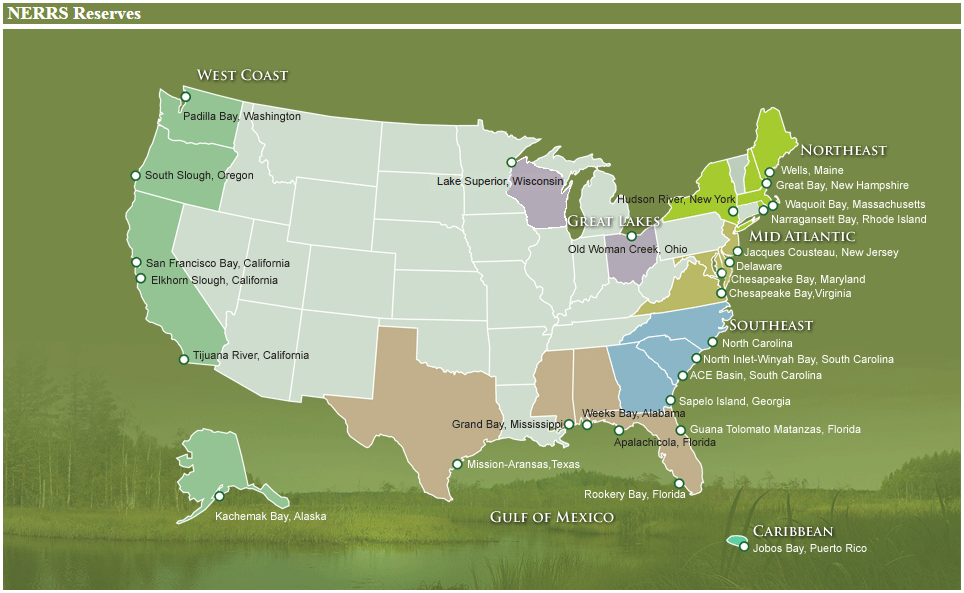
\includegraphics[width = 0.8\textwidth]{NERRS_locations.png}}
\tiny
\flushright
\href{http://nerrs.noaa.gov/ReservesMap.aspx}{http://nerrs.noaa.gov/ReservesMap.aspx}
\end{frame}

%%%%%%
\begin{frame}{Overview of SWMP and available data}
\onslide<1->
The first challenge in analyzing time series is obtaining the data \\~\\
SWMP data are available through the Centralized Data Management Office (\href{http://cdmo.baruch.sc.edu/}{CDMO})
\begin{center}
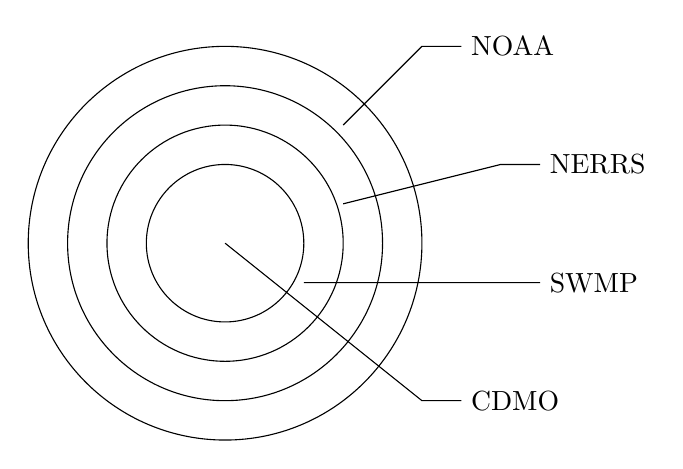
\begin{tikzpicture}[auto, >=stealth]
  \onslide<2->{
  \path
  (2,2) ellipse (2.5 and 2.5) [draw]
  (3.5,3.5) -- (4.5,4.5) -- (5,4.5) node[right]{NOAA} ;}
  \onslide<3->{
  \path
  (2,2) ellipse (2 and 2) [draw]
  (3.5,2.5) -- (5.5,3) -- (6,3) node[right]{NERRS} ;} 
  \onslide<4->{
  \path
  (2,2) ellipse (1.5 and 1.5) [draw]
  (3,1.5) -- (5.5,1.5) -- (6,1.5) node[right]{SWMP} ;} 
  \onslide<5->{
  \path
  (2,2) ellipse (1 and 1) [draw]
  (2,2) -- (4.5,0) -- (5,0) node[right]{CDMO} ;} 
\end{tikzpicture}
\end{center}

\end{frame}

%%%%%%
\begin{frame}[t]{Overview of SWMP and available data}
CDMO is your one-stop shop for retrieving SWMP data \\~\\
\centerline{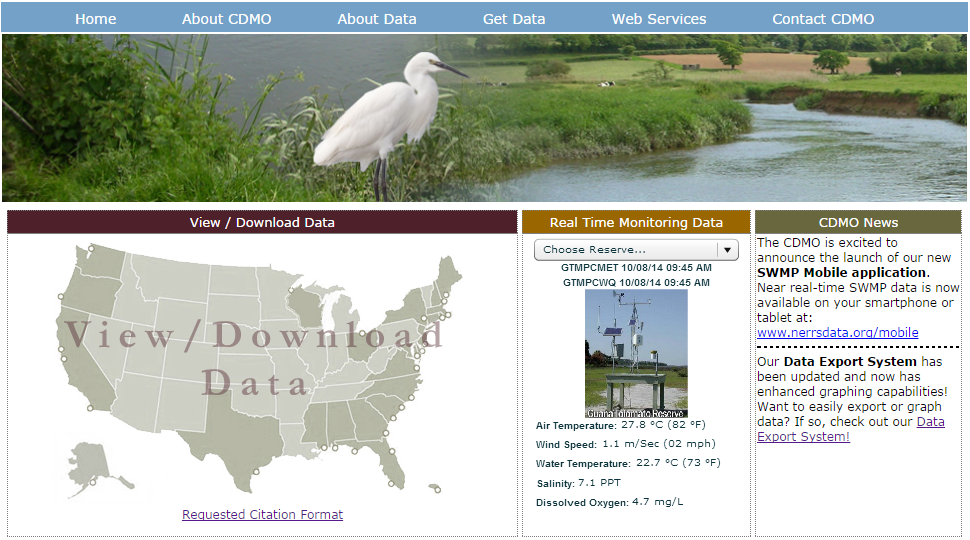
\includegraphics[width = \textwidth]{cdmo_front.png}}
\end{frame}

%%%%%%
\begin{frame}{Overview of SWMP and available data}
Data can be exported from CDMO \href{http://cdmo.baruch.sc.edu/get/landing.cfm}{several ways}:\\~\\
\centerline{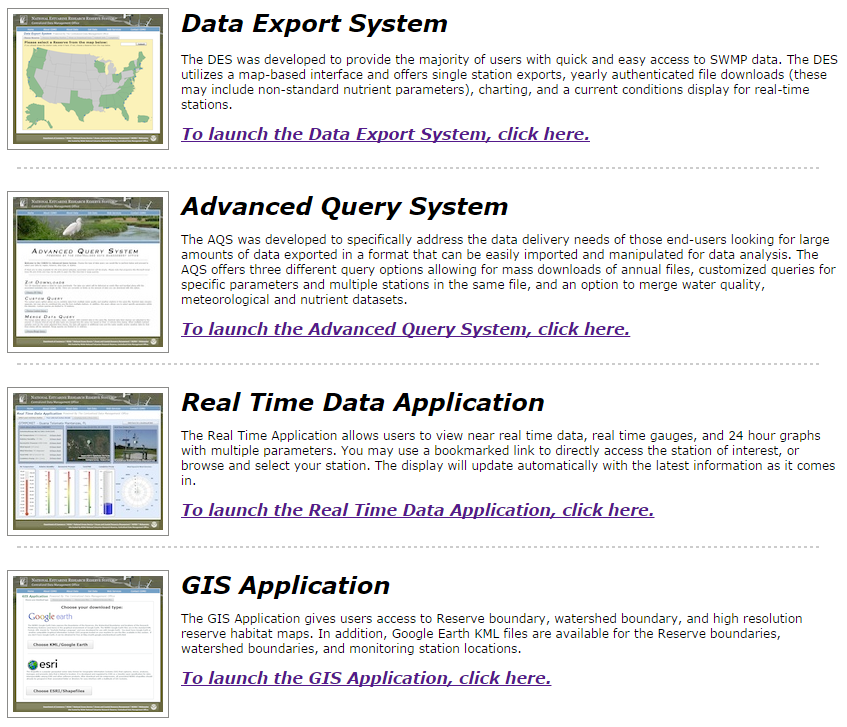
\includegraphics[width = 0.6\textwidth]{get_data.png}}
\end{frame}

%%%%%%
\begin{frame}{Overview of SWMP and available data}
A wide range of data can be requested... a few records for one site to all records for multiple sites \\~\\
Requests can return a lot of data so make sure you have clear objectives \\~\\
Check the \href{http://cdmo.baruch.sc.edu/data/availableOne.cfm}{available data} before making a request! \\~\\
\begin{itemize}
\item station names \\~\\
\item data types \\~\\
\item date ranges \\~\\
\item parameters \\~\\
\end{itemize}
\end{frame}

%%%%%%
\begin{frame}[t]{Overview of SWMP and available data}
Available data: \href{http://cdmo.baruch.sc.edu/data/availableOne.cfm}{http://cdmo.baruch.sc.edu/data/availableOne.cfm}\\~\\
\centerline{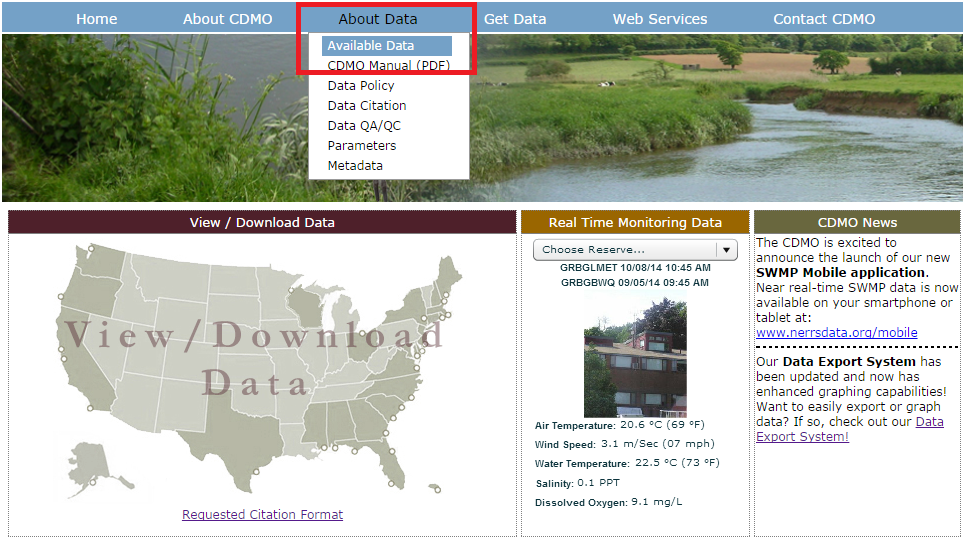
\includegraphics[width = 0.9\textwidth]{avail_dat2.png}}
\end{frame}

%%%%%%
\begin{frame}[t]{Overview of SWMP and available data}
Available data: \href{http://cdmo.baruch.sc.edu/data/availableOne.cfm}{http://cdmo.baruch.sc.edu/data/availableOne.cfm}\\~\\
\centerline{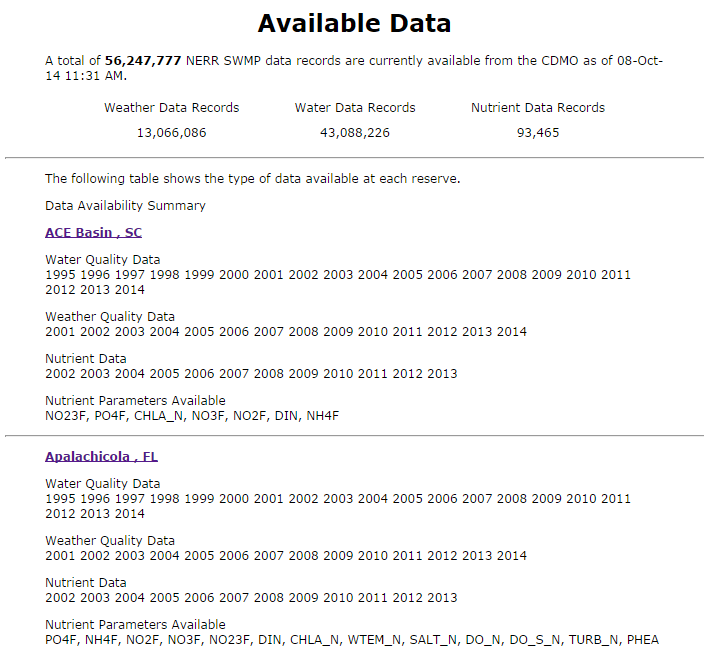
\includegraphics[width = 0.6\textwidth]{avail_dat.png}}
\end{frame}

%%%%%%
\begin{frame}[t]{Overview of SWMP and available data}
Metadata are also returned with any data request\\~\\
As `sampling\_stations.csv':\\~\\
\centerline{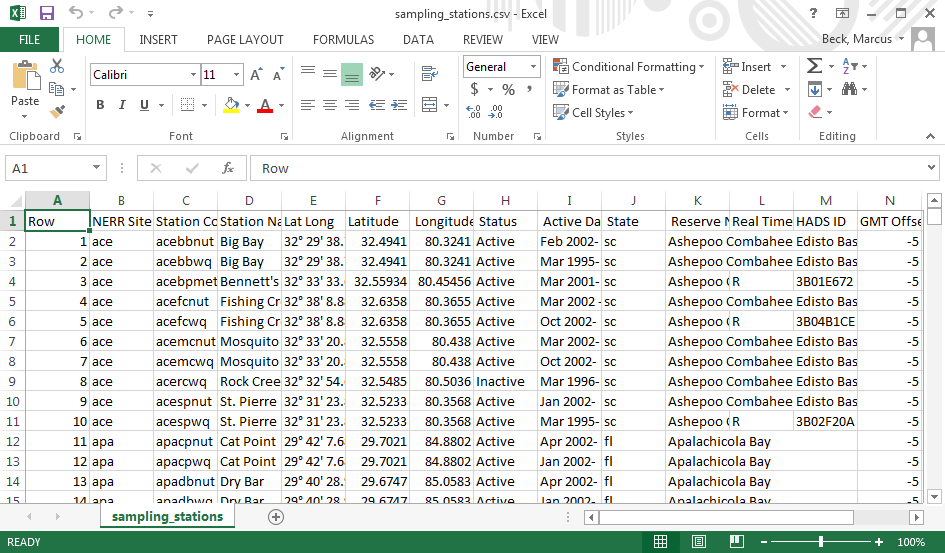
\includegraphics[width = 0.8\textwidth]{samp_stat.png}}
\end{frame}

%%%%%%
\begin{frame}[t]{Overview of SWMP and available data}
Metadata are also returned with any data request\\~\\
As Word document (e.g., `apanut01-12.03m.doc') :\\~\\
\centerline{
\includegraphics[width = 0.8\textwidth]{meta_doc.png}}
\end{frame}

%%%%%%
\begin{frame}{Overview of SWMP and available data}
The SWMP naming convention and terminology:\\~\\
Stations are identified by a 7 or 8 character name

\end{frame}

%%%%%%
\begin{frame}{Overview of SWMP and available data}
\onslide<+->
How to view available data:\\~\\
\begin{itemize}
\item Trial-and-error (not recommended)
\item View online: \href{http://cdmo.baruch.sc.edu/data/availableOne.cfm}{http://cdmo.baruch.sc.edu/data/availableOne.cfm}
\item View after request: `sampling_stations.csv'
\item View after request: year and station specific .doc file
\item Retrieve from within R (will cover later) \\~\\
\end{itemize}
\onslide<+->
\centerline{\emph{Now that you have the data, what do they look like?}} 
\end{frame}

%%%%%%
\begin{frame}{Format and potential issues with output data}

\end{frame}

%%%%%%
\begin{frame}

\end{frame}

%%%%%%
\begin{frame}

\end{frame}

%%%%%%
\begin{frame}

\end{frame}

%%%%%%
\begin{frame}

\end{frame}

\end{document}
